\documentclass[11pt, oneside]{article}   	% use "amsart" instead of "article" for AMSLaTeX format
\usepackage{geometry}                		% See geometry.pdf to learn the layout options. There are lots.
\geometry{letterpaper}                   		% ... or a4paper or a5paper or ... 
%\geometry{landscape}                		% Activate for for rotated page geometry
%\usepackage[parfill]{parskip}    		% Activate to begin paragraphs with an empty line rather than an indent
\usepackage{graphicx}				% Use pdf, png, jpg, or eps� with pdflatex; use eps in DVI mode
								% TeX will automatically convert eps --> pdf in pdflatex		
\usepackage{amssymb}
\usepackage{amsmath}
\usepackage{parskip}
\usepackage{color}
\usepackage{hyperref}

\title{Charged wire and sheet}
%\author{The Author}
%\section{}
%\subsection*{}
\date{}							% Activate to display a given date or no date

\graphicspath{{/Users/telliott_admin/Dropbox/Tex/png/}}
% \begin{center} 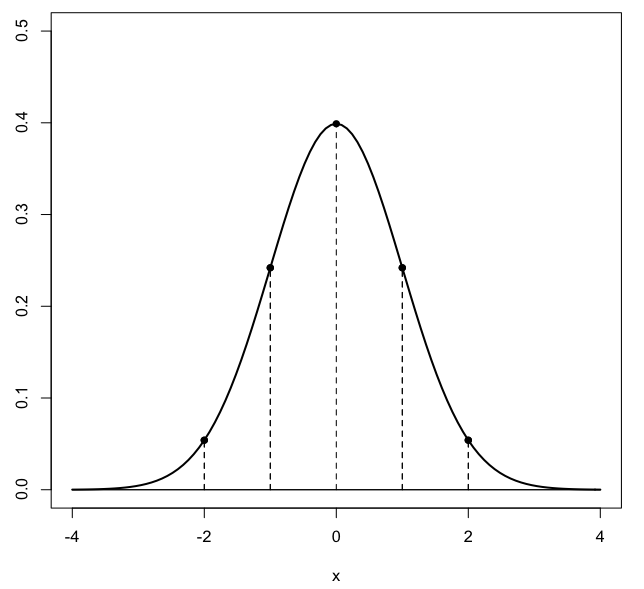
\includegraphics [scale=0.4] {gauss3.png} \end{center}
\begin{document}
\maketitle
\Large
These are two classic problems.  Find the field for an infinite wire charged with density $\lambda$ or an infinite sheet charged with density $\sigma$ (positive charge).  Start with the wire.
\subsection*{infinite wire}
\begin{center} 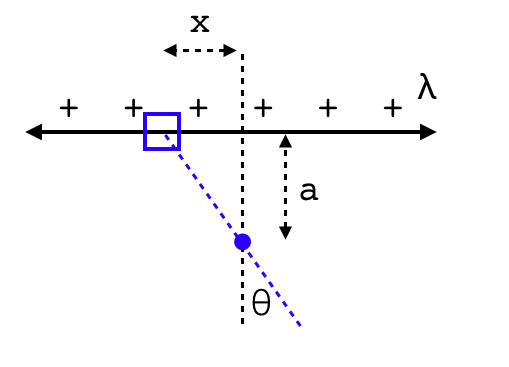
\includegraphics [scale=0.5] {charge_density1.png} \end{center}
Consider a point at a distance $a$ from the wire.  Call the nearest position on the wire $x=0$.  The force from a small element at position $x$ points radially away from the element.  Break that force into two components, the component horizontal in the figure will be canceled by a component in the other direction from its counterpart at $-x$.  The vertical component is $\mathbf{F} \cos \theta$.

Coulomb says that
\[ E = \frac{q}{4 \pi \epsilon_0} \frac{1}{d^2} \]
If the small element has width $dx$ and the density is $\lambda$, the total charge in that element is $\lambda dx$.  The distance from the element to the position we are evaluating is $\sqrt{x^2 + a^2}$.  So the small part of the electric field is
\[ dE = \frac{\lambda}{4 \pi \epsilon_0} \frac{dx}{(a^2 + x^2)} \]
There is a further factor of $\cos \theta$ to account for the fact that only the vertical part of the force is not canceled.
\[ \cos \theta = \frac{a}{\sqrt{a^x + x^2}} \]
\[ dE = \frac{\lambda a}{4 \pi \epsilon_0} \frac{dx}{(a^2 + x^2)^{3/2}} \]
To integrate this, we need a trig substitution.  Because of the $a^2 + x^2$, choose the tangent:
\[ x/a = \tan \theta \]
\[ x = a \tan \theta \]
\[ dx = a \sec^2 \theta \ d \theta \]
\[ a/\sqrt{a^2 + x^2} = \cos \theta \]
\[ \frac{1}{(a^2 + x^2)^{3/2}} = \frac{\cos^3 \theta}{a^3} \]
\[ dE = \frac{\lambda a}{4 \pi \epsilon_0} a \sec^2 \theta \ \frac{\cos^3 \theta}{a^3} \ d \theta \]
\[ dE = \frac{\lambda}{4 \pi \epsilon_0} \frac{\cos \theta}{a} \ d \theta \]
\[ E = \int \frac{\lambda}{4 \pi \epsilon_0} \frac{\cos \theta}{a} \ d \theta \]
\[ = \frac{\lambda}{4 \pi \epsilon_0} \ \frac{1}{a} \sin \theta \]
The limits require care.    The original limits on $x$ were (for an infinite wire) $x = -\infty \rightarrow \infty$.  Now $x = \tan \theta$, so $\theta = -\pi/2 \rightarrow \pi/2$.  Evaluating $\sin \theta$ between those limits we get $1 - -1 = 2$.
\[ E = \frac{\lambda}{2 \pi \epsilon_0} \ \frac{1}{a} \]
So the field falls off like $1/a$ rather than $1/a^2$.  We visualize the electric field lines as being perpendicular to the wire.  If we take a cross-section in the perpendicular plane, the field lines spread like $1$ over the distance.  It is a one-dimensional spreading.
\subsection*{infinite sheet}
\begin{center} 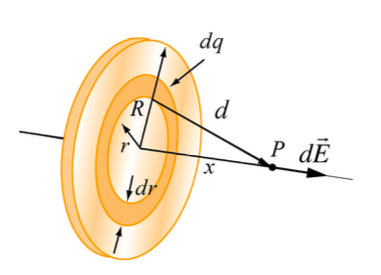
\includegraphics [scale=0.6] {charge_density2.png} \end{center}
Again, we evaluate the field at a point a distance $a$ away from the sheet.  The charge density is $\sigma$.  We think about a ring with radius $r$ centered on the position that is closest to the point where we're conducting the evaluation.  The normal vector passes through the center of the ring and through our point.

The force is directed from each little segment on the ring toward the point, but the part of the force that is not perpendicular is canceled in each case, by an opposite component coming from the piece of the ring opposite to the segment we're considering.  So again, we will have a factor of $\cos \theta$.

The distance is $\sqrt{a^2 + x^2}$ and $\cos \theta = a/ \sqrt{a^2 + x^2}$, as in the last problem.
\[ dE = \frac{dq}{4 \pi \epsilon_0} \frac{1}{d^2} \]
The ring has width $dr$ and length $2 \pi r$, so it has area $2 \pi r \ dr$ and charge $2 \pi r \sigma \ dr$.  We have
\[ dE = \frac{2 \pi r \sigma}{4 \pi \epsilon_0} \frac{a}{(a^2 + r^2)^{3/2}} \ dr \]
\[ dE = \frac{a \sigma}{2 \epsilon_0} \frac{r}{(a^2 + r^2)^{3/2}} \ dr \]
The denominator is similar to what we had in the first problem, but now we have $r \ dr$ up top.

The integral is
\[ E = \int dE = \frac{a \sigma}{2 \epsilon_0} (-\frac{1}{(a^2 + r^2)^{1/2}} ) \]
We evaluated between $r = 0 \rightarrow \infty$.  The term in parentheses becomes $- - 1/\sqrt{a^2}$, so the answer is finally
\[ E  = \frac{\sigma}{2 \epsilon_0} \]
The field is independent of $a$.  If we take a cross-section in the perpendicular plane, the field lines do not spread out.

(To do:  follow Fitzpatrick pg 41+ and show that this follows from symmetry and Gauss's Law).

\subsection*{sphere}
The problem of the sphere comes up in gravitation as well as electrostatics.  We will sidestep the determination of how a sphere or a solid ball behaves.  (See the short write-up on the shell theorem, due to Newton).  We will instead use Gauss's Law, which says the total electric flux through a surface enclosing a charge $Q$ is
\[ \Phi_E = \frac{Q}{\epsilon_0} \]
The flux is defined to be the dot product of the electric field with the surface element, integrated over the entire surface.
\[ \Phi_E = \iint_S \mathbf{E} \cdot d \mathbf{A} \]
If we have a sphere, it is symmetric in all 3 directions in Cartesian coordinates, for example.  Therefore, we expect that the electric field will be perpendicular to the surface of the sphere, and to any (imaginary) sphere that we might draw around the sphere at a radius $r$ from the center.  This means that the dot product is just $E dA$, so
\[ \Phi_E = \iint_S E dA = E \iint_S dA = 4 \pi r^2 E \]
\[ \frac{Q}{\epsilon_0} = 4 \pi r^2 E \]
\[ E = \frac{1}{4 \pi \epsilon_0} \frac{Q}{r^2} \]
\[ \mathbf{E} = \frac{1}{4 \pi \epsilon_0} \frac{Q}{r^2} \ \hat{\mathbf{r}} \]
\[ \mathbf{F} = q\mathbf{E} = \frac{1}{4 \pi \epsilon_0} \frac{qQ}{r^2} \ \hat{\mathbf{r}} \]


\end{document}  